\subsubsection{Herkunft der vertonten Texte}

\hypertarget{RefHeadingToc100333743}{}Nur bei 6 seiner Kompositionen mit
deutschem Text gibt Högn jeweils den entsprechenden Autor an. Die Texte
stammen von Schwester M. Irmingard, Hühnlein, Dr. Anton Götz, Otto
Schaffner, Hans Trohsbach, und Cordula Peregrina. Vier von Högns
Kompositionen haben ihren Text mit Werken aus dem Notenmaterial der
Pfarrei Ruhmannsfelden gemeinsam, wie folgender Tabelle zu entnehmen
ist:

\begin{flushleft}
\tablefirsthead{}
\tablehead{}
\tabletail{}
\tablelasttail{}
\begin{supertabular}{|m{5.743cm}|m{2.299cm}|m{7.6210003cm}|}
\hline
{\bfseries Komposition von Högn} &
\multicolumn{2}{m{10.12cm}|}{{\bfseries Komposition aus dem
Notenbestand}}\\\hline
Marienlied Nr. 4 G-Dur op. 23 &
Josef Gruber &
Nr. 1 aus „Zwei Marienlieder op. 221“\\\hline
Marienlied Nr. 7 G-Dur op. 45 &
Josef Gruber &
Nr. 4 aus „Marienstrauß op. 223 Heft 2“\\\hline
Kommunionlied Nr. 2 C-Dur op. 37 &
Max Welcker &
Nr. 1 aus „6 Kommunionlieder op. 89“\\\hline
Kommunionlied Nr. 3 G-Dur op. 21 &
Max Welcker &
Nr. 4 aus „6 Kommunionlieder op. 89“ \\\hline
\end{supertabular}
\end{flushleft}
Josef Gruber und Max Welcker geben ebenfalls keinen Autor an. Deshalb
war es für Högn logischerweise unmöglich, Angaben über den Autor zu
machen. Den Text zu zwei Marienliedern hat Högn selbst verfasst. Bei 12
von den insgesamt 24 deutschen Liedern Högns bleibt die Frage nach der
Herkunft des Textes aber ungeklärt. Auch nach Aussage von Barbara
Essigmann zu urteilen, \footnote{Interview Nr. 5, Barbara Essigmann,
2.1.2003, Absatz 12} könnte Högn deshalb weit mehr als nur zwei Texte
selbst verfasst haben.

\begin{flushleft}
\tablefirsthead{}
\tablehead{}
\tabletail{}
\tablelasttail{}
\begin{supertabular}{m{7.589cm}m{7.4040003cm}}

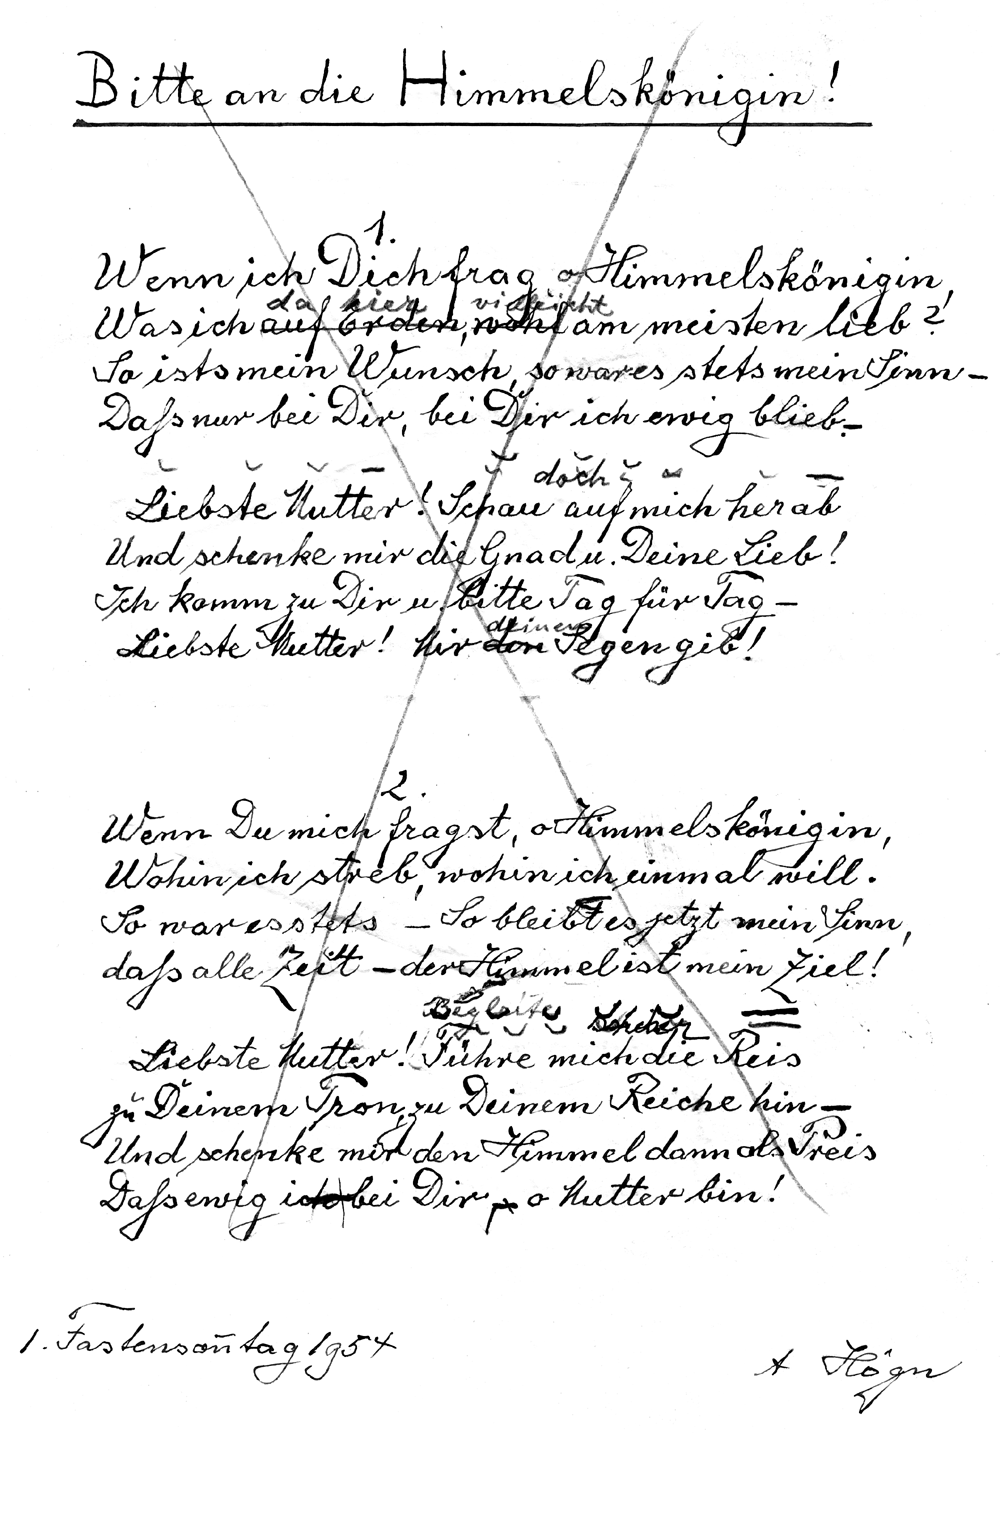
\includegraphics[width=7.408cm,height=10.964cm]{pictures/zulassungsarbeit-img069.png}

Abb. \stepcounter{Abb}{\theAbb}: Liedtext „Bitte an die Himmelkönigin!“
zum Marienlied Nr. 12 F-Dur op. 63 &

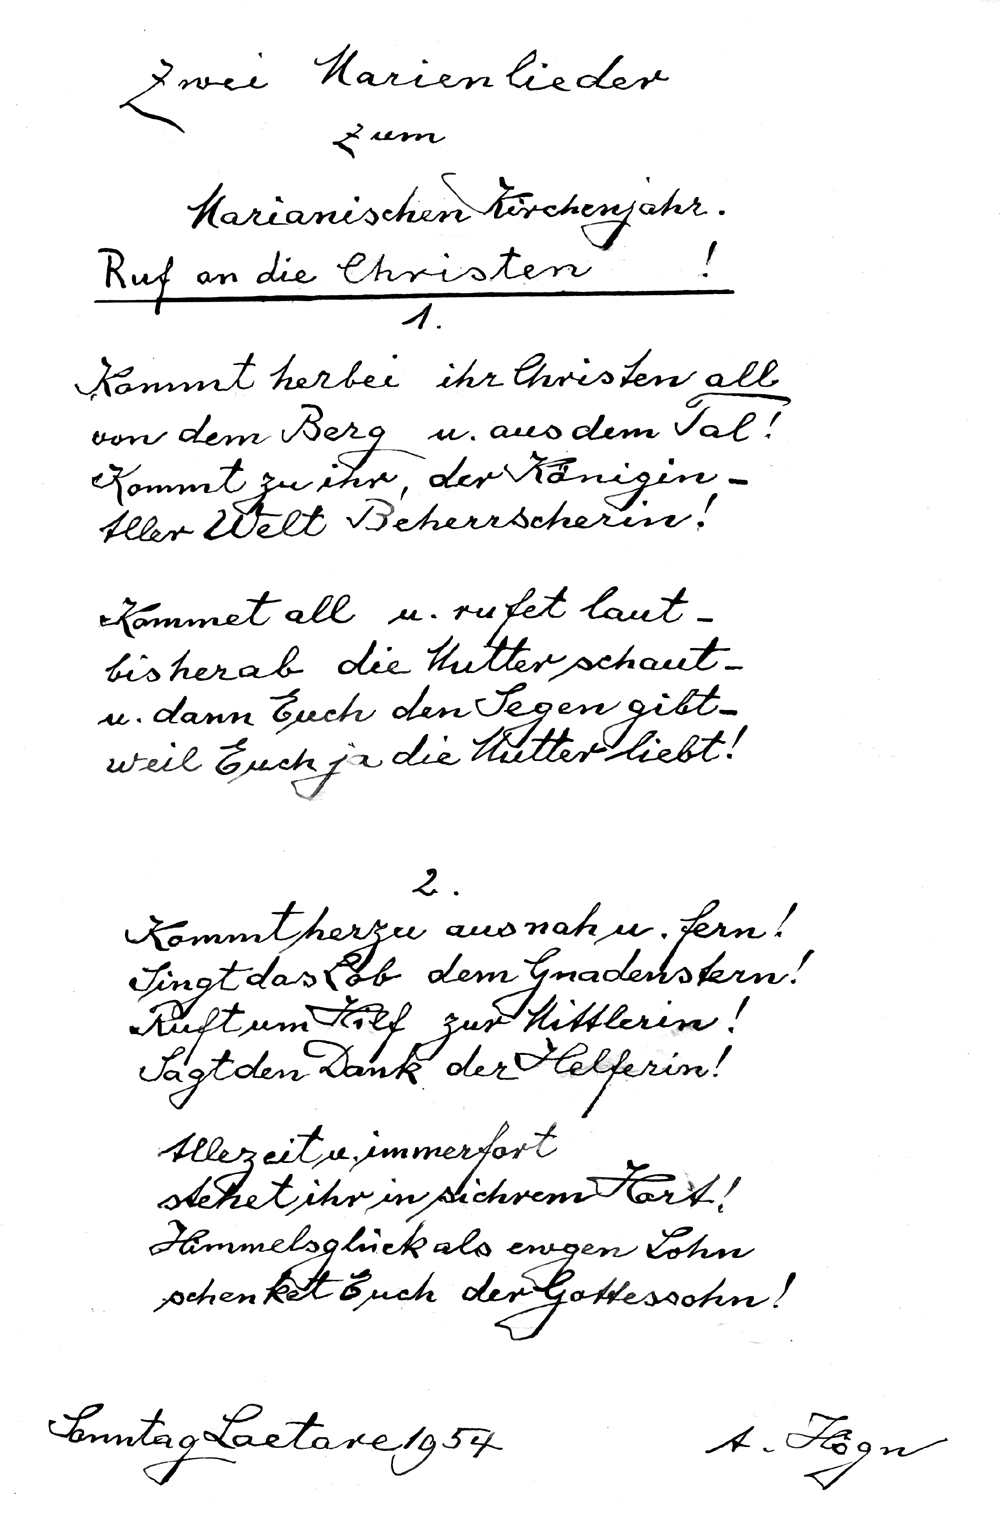
\includegraphics[width=7.223cm,height=10.964cm]{pictures/zulassungsarbeit-img070.png}

Abb. \stepcounter{Abb}{\theAbb}: Liedtext „Ruf an die Christen!“ zum
Marienlied (Nr. 13) C-Dur\\
\end{supertabular}
\end{flushleft}
Zu einer zuverlässigen Aussage, ob Högn noch weitere Texte verfasst hat,
kann man kommen, wenn man die Machart der beiden eindeutig von Högn
stammen Gedichte mit den Texten von unbekannter Urheberschaft
vergleicht. Bei den zwei von ihm verfassten Gedichten zeigt sich Högn
eher als ungeschickter Literat. Der Liedtext „Bitte an die
Himmelkönigin!“ zum Marienlied Nr. 12 F-Dur op. 63 (siehe Band II,
Seite 95) weist in drei Verszeilen, nämlich Zeile 5, 8 und 13 eine
Unterbrechung des jambischen Versmaßes auf. Insgesamt scheinen die
Verszeilen viel zu lang gewählt worden zu sein. Einerseits verblasst
dadurch der Effekt des Reimes, andererseits konnten die langen Zeilen
nicht immer mit einer sinnvollen Aussage gefüllt werden. Um die
erforderliche Silbenzahl der Zeilen „So ist´s mein Wunsch, so war es
stets mein Sinn“ (Zeile 3) oder „wohin ich streb, wohin ich einmal
will“ (Zeile 10) zu erreichen, musste Högn sogar seine Aussage in wenig
abgewandelter Form wiederholen. Beim Liedtext „Ruf an die Christen!“
des Marienlieds (Nr. 13) C-Dur (siehe Band II, Seite 95) können zwar
keine Fehler im Metrikfluss oder im Reimschema festgestellt werden,
dafür verstärkt der sehr einfache Aufbau aus Paarreim und trochäischem
Versmaß den trivialen Gesamteindruck des Gedichtes. Die Gedichte von
ungeklärter Herkunft wirken weit flüssiger und eleganter als die zwei
von Högn verfassten Texte. Man kann deshalb davon ausgehen, dass Högn
tatsächlich nur die oben besprochenen Texte geschrieben hat.

Ein Skizzenblatt zur dritten Strophe des Grablieds Nr. 3, das unter dem
Notenmaterial der Grabliedes zu finden war, zeigt, dass Högn sehr wohl
übernommene Gedichte seinen Bedürfnissen anpasste und Veränderungen
vornahm. Der Text zum Grablied von Nr. 3 stammt von Dr. Anton Götz.
Högn könnte die dritte Strophe hinzugefügt haben oder zumindest
verändert haben. Zwei andere Texte zeigen Unregelmäßigkeiten im Aufbau,
wie sie nur durch eine nachträgliche Veränderung verursacht worden sein
könnten.

\begin{center}
\begin{minipage}{10.264cm}
\begin{flushleft}
\tablefirsthead{}
\tablehead{}
\tabletail{}
\tablelasttail{}
\begin{supertabular}{m{10.064cm}}

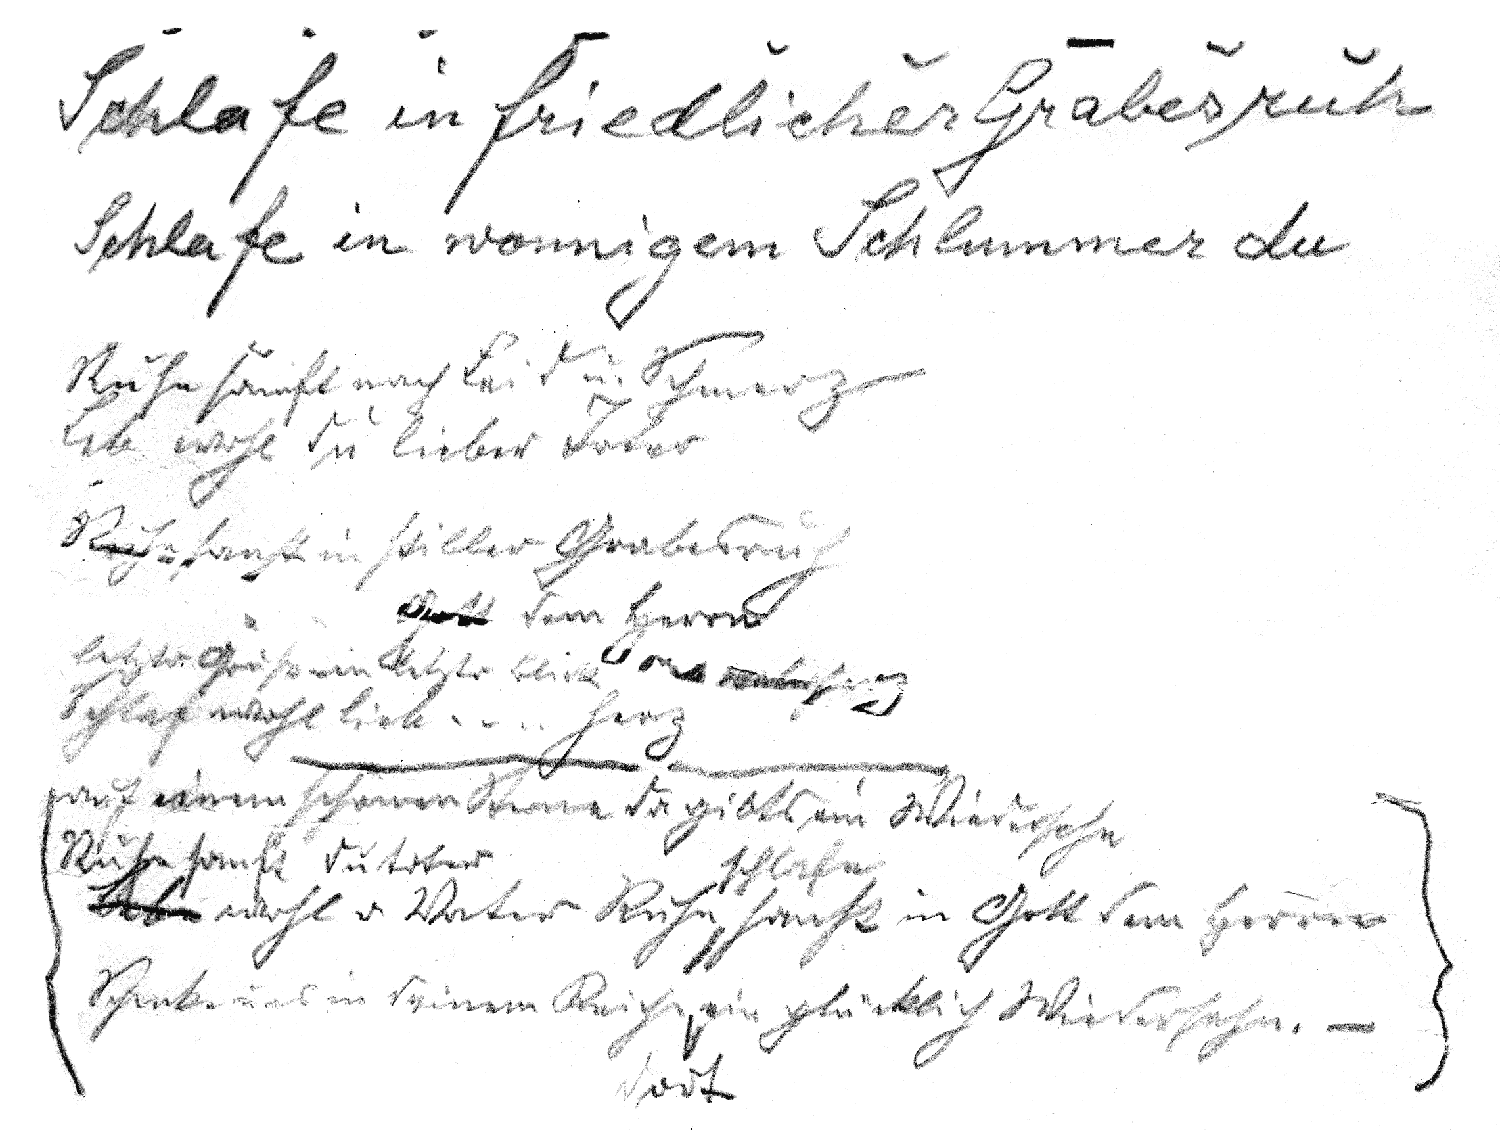
\includegraphics[width=9.881cm,height=5.323cm]{pictures/zulassungsarbeit-img071.png}

Abb. \stepcounter{Abb}{\theAbb}: Skizze zur 3. Strophe des Grablieds Nr.
3 Es-Dur op. 44\\
\end{supertabular}
\end{flushleft}
\end{minipage}
\end{center}
Die ersten fünf Textzeilen des Marienlieds Nr. 3 F-Dur op. 22 (siehe
unten) weisen ein ungewöhnliches, aber trotzdem nachvollziehbares
Reimschema und ein sehr gleichmäßiges Versmaß, bestehend aus jeweils
drei Jamben, auf. Der darauffolgende Refrain durchbricht beide Regeln.
Wie unten angedeutet, könnte Högn große Textteile eingefügt haben, um
genügend Text für das groß angelegte Wechselspiel zwischen Sopransolo
und Chor im Refrain des Marienlieds Nr. 3 ab Takt 13 bis zum Schluss zu
haben (siehe Band III, Seite 74 – 76).

\begin{flushleft}
\tablefirsthead{}
\tablehead{}
\tabletail{}
\tablelasttail{}
\begin{supertabular}{m{7.9230003cm}m{7.9230003cm}}
Text zum Marienlied Nr. 3 F-Dur op. 22 „Bitte an Maria“\newline
\newline
1. Maria, süße Mutter, \newline
du Jungfrau rein und mild.\newline
Ich komm zu dir in Schmerzen \newline
und fleh aus vollem Herzen\newline
vor deinem heilgen Bild:\newline
\textit{Maria, (reine Gottesbraut, \newline
Maria, du Reine, du) hehre Königin,\newline
(bei deinem Sohn, bei deinem gütgen Sohne,) \newline
sei du mir Schutz und Mittlerin.} &
2. O lenke meine Schritte, \newline
zu dir mich treulich führ.\newline
Auf allen Erdenwegen\newline
sei du mir Himmelssegen, \newline
mein Heil, mein Schutzpanier. \newline
\textit{Maria, hehre Königin,\newline
sei  }\textbf{du}\textit{ mir Schutz und Mittlerin.}\\
\end{supertabular}
\end{flushleft}
Auch die zweite Strophe des Grablieds Nr. 1 Es-Dur op. 35 von Otto
Schaffner weist Unregelmäßigkeiten im Vergleich zur ersten Strophe auf
(siehe unten). Im Gegensatz zur ersten ist in der zweiten Strophe kein
Reimschema mehr zu erkennen. Das Reimpaar „Welt / durchgellt“ wirkt
auch deswegen so plump, weil das Wort „Welt“ in den ersten Zeilen
zweimal wiederholt wird. Des Weiteren stimmt die Anzahl der Silben in
drei Zeilen nicht mit den entsprechenden Zeilen der ersten Strophe
überein. Es ist deshalb sehr wahrscheinlich, dass August Högn diese
zweite Strophe ergänzt hat. Das Grablied Nr. 1 hat zwei verschiedene
Textfassungen. Je nach Text fungiert das Grablied bei gleich bleibender
Musik einmal als Grablied für gefallene Krieger und einmal als Grablied
für normale Sterbefälle. Es existieren insgesamt vier verschiedene
Strophen zu einer Komposition. Vielleicht hat Högn, als er aus einem
Krieger-Grablied ein gewöhnliches Grablied gemacht hat, eine weitere
Strophe hinzugefügt und offenbar die Beibehaltung der Silbenanzahl und
des Reimschemas nicht berücksichtigt. Unter seine Komposition im
3/4-Takt (siehe Band III, Seite 80 – 81) ließen sich auch sehr flexibel
Verszeilen mit unterschiedlicher Länge einfügen. Da die Zeile „Labsal
der Sterbenden“ besonders kurz ist, wird das Wort „Labsal“ über zwei
Takte gesungen. Vielleicht hat Högn die Zeile deshalb zu kurz gewählt,
um den Effekt der Dehnung beim Wort „Labsal“ zu erreichen und so einen
besonderen Ausdruck zu gewinnen.

\begin{flushleft}
\tablefirsthead{}
\tablehead{}
\tabletail{}
\tablelasttail{}
\begin{supertabular}{m{7.9230003cm}m{7.9230003cm}}
Text zum Grablied Nr. 1 Es-Dur op. 35 (normale Sterbefälle)

Schlafe in friedlicher Grabesruh, (9 Silben)\newline
schlafe in wonnigem Schlummer du. (9)\newline
Selig, selig der Welt entrückt, (8)\newline
schauen wirst du das Himmelslicht, (8)\newline
da der ewige Tag anbricht. (8)\newline
Selig, selig von Gott beglückt. (8) &
Schaurig und kalt steht vor uns die Welt. (9)\newline
Trauer und Klagen die Welt durchgellt. (9)\newline
Heiland, Heiland, o Heiland der Welt, \textbf{(9)}\newline
All unser Glück und Trost im Leid, (8)\newline
Labsal der Sterbenden, \textbf{(6)}\newline
Freund der Toten, o Heiland, bist du. \textbf{(9)}\\
\end{supertabular}
\end{flushleft}





